\section{Theoretical introduction}
Light interacting with matter is still one of the most important aspects of physics, including
absorption, emission, but also scattering. In this report we will guide our attention to one
particular form of light interaction: \textit{Raman scattering}, which is widely used in spectroscopy
in many different areas, from applied chemistry to aerospace engineering. We will illustrate the 
basic functionalism through a series of simple experiments.

\subsection{Classical description}
\label{sub:classical_description}

\subsubsection{Oscillation of molecules}
\label{ssub:Oscillation_of_molecules}
Let us first investigate~\cite{landau1997mechanik} the classical oscillation of molecules, their normal modes and how a classical 
electric field interacts with them. When talking about a system of particles interacting with each other, not all degrees
of freedom will be oscillatory behavior. In general for a n-atomic molecule 
the dimension of the oscillation will be $3n - 6$ and $3n -5$ for a linear molecule (lying on a line), since three for
translation and three rotation of the whole molecule are subtracted. Now let us remove these 6 (5) dimensions from the
equation of motion and transform into the rotation and move less center of mass system:
\begin{equation}
    \sum_a m_a r_a = \mathrm{const} \equiv \sum_a m_a r_{a,0}.
\end{equation}
Using new coordinates, we express this condition as
\begin{equation}
    \sum_a m_a x_a = 0.
\end{equation}
This conditions out coordinates with respect to translation, now we need to find a constraint
to remove the rotations. Let us look at the angular momentum $\mu$: 
\begin{equation}
    \mu = \sum_a m_a r_a \times v_a \approx \sum_a m_a r_{a 0} \times \dot{x}_a = \frac{\partial}{\partial t}
    \sum_a m_a r_{a 0} \times u_a
\end{equation}
where we only look at small deviations $r_a = r_{a0} + x_a$. We can let it vanish if we demand
\begin{equation}
    \sum_a m_a r_{a0} \times x_a = 0.
\end{equation}
Remember that $u$ characterizes the inherent oscillations out of center of mass. Let us now
look at the energy of the molecule. Let a potential energy $U$ lead to the oscillation around zero,
then we can approximate it as a quadratic form with coefficients $k_{ik}$ (a generalized, coupled
harmonic oscillator):
\begin{equation}
    U = \frac{1}{2} \sum_{i,k} k_{ik} x_i x_k
\end{equation}
Hence the total energy becomes:
\begin{equation}
    E = \frac{1}{2} \sum_{i,k} m_{ik} \dot{x}_i\dot{x}_k + \frac{1}{2} \sum_{i,k} k_{ik} x_i x_k   
\end{equation}
with a linear transformation we can go into the uncoupled \textit{normal coordinates} $q$:
\begin{equation}
    E = \frac{1}{2} \sum_{i,a} \dot{q}^2_{ai} + \frac{1}{2} \sum_a \omega_a^2 \sum_i q^2_{a,i} 
\end{equation}
Where as before $a$ goes over the different modes and $i$ over the spatial dimensions.
Let us go back to the coordinates $x$ and look at the solution of the classical equation
of motion. The Lagrange function reads
\begin{equation}
    L = \frac{1}{2} \sum_{i,k} (m_{ik} \dot{x}_i\dot{x}_k -  k_{ik} x_i x_k   )
\end{equation}
The partial derivatives become 
\begin{equation}
    \frac{\partial L}{\partial \dot{x}_i} = \sum_k m_{ik} \dot{x}_k , \quad 
    \frac{\partial L}{\partial x_i} = - \sum_k k_{ik} x_k.
\end{equation}
The \textit{Euler Lagrange} equation is then 
\begin{equation}
    \label{eq:el}
    \sum_k (m_{ik} \ddot{x_k} + k_{ik} x_k) = 0 
\end{equation}
This is a linear matrix differential equation which can be solved in terms of exponentials
\begin{equation}
    x_k = A_k \exp(i\omega t).
\end{equation}
so~\eqref{eq:el} becomes
\begin{equation}
    \sum_k \left( -\omega^2 m_{ik} + k_{ik} \right)A_k = 0
\end{equation}
which finally give rise to the eigen frequencies $\omega$
\begin{equation}
    |k_{ik} - \omega^2 m_{ik}| = 0. 
\end{equation}
Fortunately, it is not necessary to calculate those in every case, since
molecules are often governed by easy symmetries. The task simplifies to
find the respective symmetry group and its irreducible representations~\cite{landau1977quantum}. 


\subsubsection{Electric fields and dipoles}
\label{ssub:Electricfieldsanddipoles}
Let us examine classical electromagnetic waves. The solution to the homogeneous
wave equation in cylindrical coordinates reads
\begin{equation}
    E(x,t) = |E| \textrm{Re} \left[ \begin{pmatrix}
            \cos(\theta)\exp(i \alpha_x)\\ 
            \sin(\theta)\exp(i \alpha_y)
    \end{pmatrix}\exp(i(kz - \omega t))  \right].
\end{equation}
The phases $\alpha_x$ and $\alpha_y$ characterize the polarization. If the polarization
is linear, the condition is
\begin{equation}
    \alpha_x = \alpha_y 
\end{equation}
The radiation field $E$ of a dipole
can be described with the dipole moment $\mu$ and in terms of the electric potential $\phi$
\begin{equation}
\phi \approx \frac{\mathbold{\mu}\cdot \mathbold{R}}{4\pi\epsilon_0 R^3} \Rightarrow E = - \nabla \phi 
= \frac{3 \mathbold{(\mu \cdot n) n - \mu}}{4 \pi \epsilon_9 R^3}.
\end{equation}
with the unit vector $\textbf{n} = \frac{\textbf{R}}{R}$. We can use this knowledge now for 
generalization.
Beginning with a Hertzian dipole~\cite{koningstein1972introduction}, the total intensity
per second can be expressed in terms of the radiation field of the dipole 
\begin{equation}
    \label{eq:hertz}
   I = \frac{2}{3 c^2} \left \langle \frac{\mathrm{d}^2}{\mathrm{d} t^2}  \mu \right \rangle_t.
\end{equation}
Where the brackets denote to the time average and $\mu$ is the electric dipole moment. Let us assume,
we induce a dipole by an incoming electric field (for instance a vibrating molecule).
Then the dipole can in general be written in terms of the electric field $E$ with
\begin{equation}
    \label{eq:mu}
    \mu_i = \sum^{3}_{j=1} \alpha_{ij} E_j(t) \equiv \alpha_{ij} E^j 
\end{equation}
with the polarization tensor $\alpha$, which describes the polarizability of the molecule.
It has to be a tensor, because otherwise the description would not be as general as possible.
Consider for instance the case of scalar $\alpha$, then the orientation of the molecule
would not have any effect on the polarizability, which is not true in most of the cases (only
if the molecule is isotropic).
Let us assume now a incoming plain wave 
\begin{equation}
    E_j = E^0_j \cos(\omega_L t).
\end{equation}
For an isotropic molecule this is an scalar and we get
for the intensity by~\eqref{eq:hertz}:
\begin{equation}
    \label{eq:I}
    I = \frac{16 \pi^4 c}{3 \lambda_0^4} \alpha ^3 E_0 ^2
\end{equation}
with $\lambda_0 = c/ 2\pi \omega_L$. Transforming into normal coordinates $q(t)$ we can write down the polarization tensor
in a Taylor expansion around zero\cite{ver}:
\begin{equation}
    \alpha = \alpha_0 + \frac{\partial\alpha}{\partial q}q(t) + \cdots \approx \alpha_0 + \alpha' q_0 \cos(\omega_M t).
\end{equation}
Where we approximated the vibration of the isotropic molecule by a frequency $\omega_M$.
The dipole moment then becomes\footnote{Where we used the trigonometric relation
\begin{equation*}
    \cos\alpha \cos\beta = \frac{1}{2}\left( \cos(\alpha +\beta) + \cos(\alpha -\beta) \right)
\end{equation*}
}

\begin{align}
    \mu &= \alpha_0 E^0 \cos(\omega_L t) + \alpha' E^0 \cos(\omega_L t) \cos(\omega_M t) \\
        &= \alpha_0 E^0 \underbrace{\cos(\omega_L t) }_{\text{Rayleigh}}
    + \alpha' E^0( \underbrace{\cos((\omega_L + \omega_M)t ) }_{\text{Anti-Stokes}}
    + \underbrace{\cos((\omega_M - \omega_L)t)}_{\text{Stokes}} ) 
\end{align}
With the emission of a \textit{Rayleigh} line and two \textit{Raman} lines (\textit{Stokes} and \textit{Anti-Stokes}).
We notice that in the classical picture here the intensity of the emitted light would be identical for both lines, which
turns out to be wrong. To explain this inequality we will need to infer quantum mechanics and statistical physics.
If we were to continue the Taylor expansion
\begin{equation}
    \alpha = \alpha_0 + \frac{\partial\alpha}{\partial q}q(t) + \frac{\partial^2\alpha}{\partial q^2}q^2(t) + \cdots
\end{equation}
We would get higher harmonics of the Raman lines, for instance $\omega_M \pm 2\omega_L, \omega_M \pm 3\omega_L$ and so
forth with less intensity at each order. 
Which is clear by now is the dependence of Raman lines of the
derivatives $\frac{\partial\alpha}{\partial q}q(t) + \frac{\partial^2\alpha}{\partial q^2}q^2(t) + \cdots$, so if 
the first one is zero
\begin{equation}
    \frac{\partial\alpha}{\partial q} = 0
\end{equation}
we will have no first order Raman lines, this is called \textbf{Raman inactive}, while the former is called
\textbf{Raman active}. 
\subsubsection{Depolarization}
\label{ssub:Depolarization}

Let us come back to the polarizability. Analogous to~\eqref{eq:I} the intensity of a fixed
dipole can be expressed as 
\begin{equation}
    I = \frac{\omega^4 \mu^2}{32\pi^2 \epsilon_0 c^3}.
\end{equation}
If the detector is fixed in x-direction, the light is polarized in z- and y-direction\cite{wiss}
\begin{equation}
    I_{z+y} = \frac{\omega^4}{32\pi^2 \epsilon_0 c^3}(\mu_z^2 + \mu_y^2)
\end{equation}
Where the $\mu_y$ and $\mu_z$ are evaluated with respect to~\eqref{eq:mu}. In general we cannot consider 
the orientation of the molecules, hence we need to look at coordinate transformation invariants of
the polarization tensor. One straightforward invariant is the trace: 
\begin{equation}
    \mathrm{Tr}( T^{-1}\alpha T) = \mathrm{Tr}(\alpha)
\end{equation}
If we look at the tensor as an ellipsoid, the trace can be seen as the mean radius: 
\begin{equation}
    \text{mean radius $\bar{\alpha}$: } \frac{1}{3}\mathrm{Tr}(\alpha) = \frac{1}{3}(\alpha_{xx} +\alpha_{yy}+ \alpha_{zz})
\end{equation}
Another invariant is
the anisotropy:
\begin{equation}
    \gamma = \frac{1}{2} \left( (\alpha_{xx} - \alpha_{yy})^2 + (\alpha_{yy} - \alpha_{zz})^2 + (\alpha_{zz} - \alpha_{xx})^2
        + 6(\alpha_{xy} + \alpha_{yz} + \alpha_{zx}) 
    \right).
\end{equation}
So if we want to examine the components the intensity, it can be shown~\cite{koningstein1972introduction} that 
\begin{align}
    I_{z} &= \frac{\omega^4}{32\pi^2 \epsilon_0 c^3} \left( \bar{\alpha}^2 + \frac{4}{45}\gamma^2 \right) E_z^2 \\
    I_{y} &= \frac{\omega^4}{32\pi^2 \epsilon_0 c^3} \left( \frac{1}{15}\gamma^2 \right) E_z^2 \\
\Rightarrow  I_{x+y} &= \frac{\omega^4}{32\pi^2 \epsilon_0 c^3} \left( \bar{\alpha}^2 + \frac{7}{45}\gamma^2 \right) E_z^2.
\end{align}
Hence the depolarization becomes:
\begin{equation}
    \rho_z =  \frac{I_z}{I_y} = \frac{3\gamma^2}{45\bar{\alpha}^2 + 4\gamma^2} 
\end{equation}
This is only valid for a linear in the z-direction polarized laser. For other configurations the 
depolarization depends strongly on the polarization direction of the laser.
%todo siehe Raman buch s.129
\subsection{Quantum mechanical treatment}
\label{sub:quantum_mechanical_treatment}
The most general treatment of the Raman effect involves scattering theory, such that we look at the incoming 
photon as a source of time-dependent perturbation on the energy levels of the molecule. Radiation emitted or absorbed is 
a result of the system making a downward or upward transition between two discrete energy levels; The virtual states only
exist as resonances, because they are a time dependent phenomenon and cannot be reduced to the stationary solution of 
the Schrödinger equation. However, we can treat them as discrete energy levels as long as they exist and calculate the
transition element. The transition moment could be defined as
\begin{equation}
    M_{fi} = \langle \psi_f | \hat{\mu} | \psi_i \rangle 
\end{equation}
with the initial and final states and the dipole moment operator\footnote{Note that this is a vector operator. This 
important, because it inherits the information about the polarization of the transition, depending on the phase factors
associated with the two states.}
$\hat{\mu}$, which takes the same
form as~\eqref{eq:mu}. Hence, we can write this the matrix element of $\hat{\mu}$ by
\begin{equation}
    \label{eq:muhat}
    \mu_{fi} = \langle \psi_f | \hat{\alpha_{kl}} | \psi_i \rangle E^k.
\end{equation}
The transition dipole moment can be used to investigate the selection rules of transitions under electric
dipole interaction, as it is the case when interfering with a classical field. Let us look at the Hamiltonian
to understand the type of interaction:
\begin{equation}
    H = \frac{p^2}{2M} + e\phi(x) - \frac{e}{mc}[A \cdot p]
\end{equation}
with the classical fields $A$ and $\phi$. The dipole approximation uses now the fact, that
the wavelength of the classical field is far longer than the molecular dimension~\cite{sakurai2011modern}.
For a transition to happen, the transition dipole moment has to be nonzero; such transitions occur between
even and odd orbitals (otherwise the integral in~\eqref{eq:muhat} gets zero). Now look at figure~\ref{fig:qm_states}
which shows the different effects: Rayleigh scattering is essentially the main event, while the two other 
lines involve another frequency (which is most commonly for molecules a vibrational state). 
\begin{figure}[htpb]
\centering
    \includegraphics[width=0.6\linewidth]{figures/qm_states.eps}
    \caption{In the quantum mechanical description we look at the Raman emission in terms of virtual energy states.
    The different lines, Stokes and Anti-Stokes, are realized by different processes.}
\label{fig:qm_states}
\end{figure}
In order to explain
the different intensities, we need to leave the purely Quantum mechanical treatment and include the many-body
statistical behavior of the states. A good approximation yields the Boltzmann distribution
\begin{equation}
    \frac{N_e}{N_a} = \exp\left (\frac{E_a - E_e}{k_B T}\right ).
\end{equation}
With the ground state $N_a$ and the first vibrational state $N_e$. This explains why the Anti-Stokes line
is of lower intensity as the Stokes line. A better approach includes the matrix element of the polarization tensor and
the degeneracy of the states~\cite{ver}. The result is 
\begin{equation}
    \frac{I_{\mathrm{Stokes}}}{I_{\mathrm{Anti-Stokes} }} = \frac{(\nu_o - \Delta \nu)^4}{(\nu_o + \Delta \nu)^4} 
    \exp \left( \frac{h\Delta \nu}{k_BT} \right)
\end{equation}
with the frequency difference 
\begin{equation}
\Delta \nu = \frac{\omega_\mathrm{S} - \omega_{\mathrm{AS}}}{2\pi c} 
\end{equation}
between Stokes and Anti-Stokes.


